\chapter{FogStore}

Situation-awareness applications maintain state, that guides the action of the application in the future. Application state consists of recently generated events (such as a vehicle detection) and location-tagged data-items (such as the state of a traffic light). Hence, system support primitives for {\it saving and retrieving events} that constitute the application state are critical in a service platform meant for geo-distributed applications. Contemporary stream processing platforms like Foglets \cite{foglets}, Apache Flink \cite{flink} and Samza \cite{samza} provide primitives for accessing and modifying the application state. Quite often, multiple application components on different edge nodes may want to share the application state -- e.g.,  situation-awareness applications may have multiple processes working on events pertaining to the same geographical area; this would require moving the state out of memory into an out-of-core external store \cite{sharedstateflink} - a design choice that is also supported by Apache Flink. Keeping such application state information on Cloud-based data stores would defeat the purpose of placing the application components in geo-distributed fog/edge nodes since saving/retrieving state is in the critical path of the application execution and should incur as little latency as possible. Hence, the application state needs to be stored in a geo-distributed manner as well \cite{confais2017performance}, leveraging the same edge nodes as those used for placing the computational components. 
\par Situation-awareness applications have stringent timing requirements on the sense-process-actuate control loop, which involves accessing application state in the critical path. To ensure that the application's control loop can operate at the desired speed, access to application state needs to be possible with low latency. Situation-awareness applications require strong consistency guarantees on the application state \cite{consistentstreaming}. In fact, researchers at Google observe that coping with eventual consistency in the application layer requires significant development time and often leads to complicated and error-prone mechanisms \cite{f1}. Hence strong consistency should be provided by the datastore layer itself. Furthermore, the application state should remain available in spite of failures of data store nodes.
\par Cloud-based data stores such as Cassandra, DynamoDB, etc. have a performant data-plane which offers low latency of data access. They also offer strong consistency guarantees along with fault-tolerance. However, Edge infrastructure poses peculiar challenges which are not present in Cloud datacenters, for which these systems are designed. Firstly, the network topology of the Edge infrastructure is highly heterogeneous, and low latency data access is only possible if the data replicas are located close to the client. Ensuring strong query consistency demands that the data replicas on which query is executed are located in proximity to the client. However, Edge infrastructure is more susceptible to geographically correlated failure, which increases the probability of making multiple replicas of a given data-item unavailable. Hence, latency, consistency and failure tolerance are conflicting objectives at the Edge, and the control-plane of off-the-shelf data stores do not offer a reasonable tradeoff between them. 
\par FogStore tackles the problem of providing both the conflicting but valid objectives of fault-tolerance and low-latency while satisfying consistency guarantees in geo-distributed key-value stores. The key insight about situation-awareness applications is the dependence of relevance of a certain data-item on the client's context. For instance, in the smart city domain, information related to a particular city may be relevant to clients who are in close proximity to that city. Using this context-sensitive characteristic of applications, we design a replication strategy that guarantees strong consistency for relevant data replicas and eventual consistency for the replicas intended primarily to ward off geo-correlated failures.  
%we trade-off globally consistent access to application state for low-latency and fault-tolerant access with strong consistency guarantees to clients for whom the data item is contextually relevant. 
The strategy is to place replicas close to the relevant clients (for low latency) and also in geographically distant locations (for fault-tolerance).
% and making a distinction in how consistent these replicas are kept. The replicas close to relevant users are kept strongly consistent, while those away are kept eventually consistent. 

{\it FogStore}, which embodies the design principles for achieving fault-tolerance and low-latency for strongly consistent access to application state makes the following contributions:
%The following points sum up the contributions of this paper :
\begin{itemize}
    \item Develop a notion of \textit{relevance} for situation-awareness applications, which is formalized as \textit{Context-of-Interest} (CoI) - which determines the degree of consistency at which queried state should be reported;
    \item FogStore utilizes the Dynamic Spatial Context Management mechanism to perform location-aware replica placement to ensure low latency data access along with tolerance from geographically correlated failures.
    \item FogStore utilizes the Dynamic Spatial Context Management mechanism to perform quorum selection that guarantees strongly consistent operations for \emph{relevant} data.
\end{itemize}
The roadmap of this chapter is as follows. \cref{sec:background} provides a background of the motivating application scenario and the basic concepts of a key-value store. It also discusses in detail the requirements of situation-awareness applications and the challenges of meeting those requirements in an Edge setting. \cref{sec:fogstore_arch} presents the architecture of FogStore. \cref{sec:replica_placement} describes how FogStore leverages the Dynamic Spatial Context Management mechanism to perform replica placement to ensure low-latency data access along with tolerance from geographically correlated failures. \cref{sec:consistency_tuning} describes how FogStore uses the same mechanism to perform quorum selection to ensure high consistency data access for \textit{relevant} data items. \cref{sec:evals} presents results of experimental evaluation of FogStore and \cref{sec:conclusion} concludes the chapter.

\section{Background}
\label{sec:background}

\subsection{Motivating Application Scenario}
\label{sec:fogstore_application}
To highlight the necessity of a system like FogStore, we present a motivating use-case that poses strict latency and staleness requirements on the data-store. Consider a distributed camera network that may be deployed on urban roadways, feeding real-time video streams for multi-camera tracking of suspicious vehicles. 

\begin{figure}
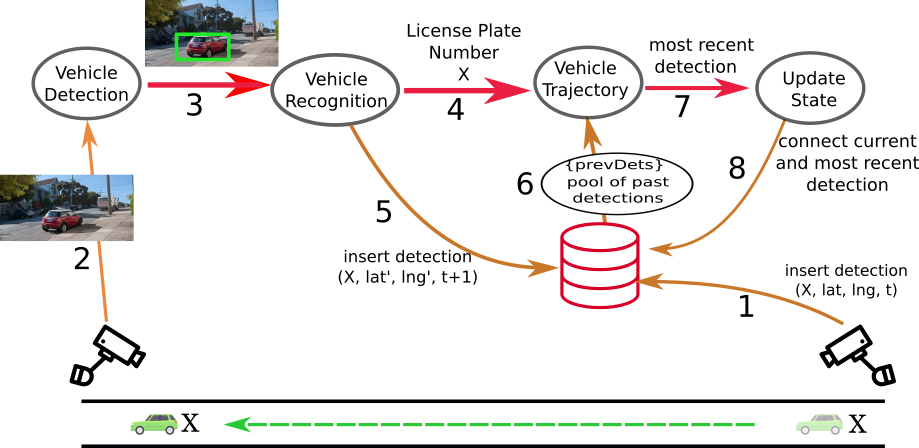
\includegraphics[width=\columnwidth]{figures/fogstore/vehicleTrackingFlow.png}
\caption{Schematic of multi-camera tracking of suspicious vehicles. The numbered arrows suggest the temporal order of flow of information.}
\label{fig:usecase-schematic}
\end{figure}

\par The application can be logically partitioned into components, as per the MobileFog programming model \cite{mobilefog}, each performing a specific function and having well-defined input-output characteristics. A schematic of the application is presented in Figure \ref{fig:usecase-schematic}. Upon detection of a vehicle in a video frame, the application extracts the identity of the vehicle by reading the license plate to get the unique identifier of the vehicle. It then inserts the detection of that vehicle along with location and time into the set of detections. The application also maintains the complete trajectory information of the vehicle, in that, for each detection of a vehicle, it saves the location and time when the car was detected before that. To achieve this, for each detection the application retrieves the set of previous detections that took place within 5 KM and 10 minutes from the current detection. It looks for the most recent detection from them and adds the identifier of that detection to the current detection's $prevDetection$ field.

\begin{algorithm}
\caption{Vehicle tracking algorithm}\label{usecasealgo}
\begin{algorithmic}[1]
\Procedure{onDetectVehicle}{V, X, Y, T}
%\State $K \gets \text{INSERT INTO vehicle\_detections} $
\State $K \gets \text{INSERT INTO vehicle\_detections} \left(V, X, Y, T \right)$
\State $prevDets \gets \text{SELECT * FROM vehicle\_detections} \newline \text{WHERE } \left( x,y \right) \text{within 5 km } \& t \text{ WITHIN 10 min ORDER BY t }$
\State $prevDet \gets k.V : k \text{ has most recent time in } prevDets$
\State $\text{UPDATE K in vehicle\_detections SET K.prevDet = prevDet}$
\EndProcedure
\end{algorithmic}
\end{algorithm}
\par It is evident from the schematic that access to application state lies in the critical path of application execution, hence making correct execution of the application contingent on fast access to state. For instance, if the insert of a vehicle detection is slow, the vehicle may be detected by an adjoining camera and not mark the former detection as the previous one - hence missing that detection from the trajectory. It is worth noting that the presented application has a dependence on contextually relevant events, specifically previous detections within a 5 km radius and at a maximum of 10 minutes before the current detection. Events that don't fall under this space-time filter may be past detections of the car but are typically not relevant for generating a fine-grained trajectory. Furthermore, retrieving the entire set of previous detections of the particular car and searching for the most recent detection could be slow. 

\subsection{Interface offered by a Key-Value Store}
\subsubsection{Data Model}
The data-model of FogStore follows a key-value pair model, wherein keys are strings and values can be elementary data-types such as strings, integers or floating point numbers, or a dictionary of key-value pairs themselves. Following are the types of key-value pairs that data-items of typical applications contain.
\begin{itemize}
\item Each data item needs to possess spatial information, that is, location in terms of latitude-longitude. This field denotes the location of the event or entity that the data-item is about.
\item Data-items, especially those that pertain to events that happened at a certain point of time, contain a timestamp field.
\item Data-items are allowed to contain key-value pairs specific to the application's logic, such as vehicle identifier in the case of a multi-camera vehicle tracking application.
\item It is up to the developer to specify which keys of a set of data-items constitute the primary key, which will be used to uniquely identify data-items for queries.
\end{itemize}

\begin{lstlisting}[caption={A sample data-item that captures a spatio-temporal event in the vehicle-tracking application's detection set. The field storing Vehicle ID forms the key that will be used to retrieve detections of a particular vehicle.},captionpos=b,label={lst:listing1},language=Json]
{
  "vehicle_id": "A54 3527",
  "location": {
    "latitude": "33.42553",
    "longitude": "-84.74456",
  },
  "timestamp": "1520123197"
}
\end{lstlisting}

\subsubsection{Types of Query Supported}
FogStore supports the following types of queries.
\begin{itemize}
\item \textbf{Insert/Delete data-items. } FogStore allows applications to insert data-items into the store by providing the key-value pairs that make up the data-item, including the primary key. For deleting a data-item the application can simply use the primary key.
\item \textbf{Update data-items. } FogStore allows applications to update an existing data-item by providing the primary key of the data-item and the new set of key-value pairs. If the key exists the value will be updated, otherwise a new key-value pair will be added to the data-item.
\item \textbf{Selecting data-items. } Applications can fetch data items whose key-value pairs match a certain predicate. The predicate can either be an exact match on one or more keys or an inequality-based condition.
\end{itemize}

\subsubsection{Replication and Consistency of Data}
\label{sec:replication}
\begin{itemize}
\item Key-value pairs which belong to the same application have keys that belong to the same keyspace. 
\item Dynamo-style data stores map data to storage nodes by computing a hash-function on the key. The output range of the hash function is divided among the storage nodes such that if a key's hash falls within the partition that is mapped to a particular storage node, then the key-value pair will be mapped to that node. 
\item Each storage node is assigned a \textit{token} on the output range of the hash function. The storage node with the smallest token that is greater than the hash value of a key is assigned as the primary replica of the key-value pair (as shown in \cref{fig:hashring_replication}). Additional replicas are chosen based on the requirements of the application (replication factor, rack-awareness, etc.) and the primary replica.
\end{itemize}

Key-value stores built on the Dynamo-style model offer fine-grained tuning options for consistency per-operation. Figure \cref{fig:hashring_replication} shows how Cassandra (a popular Dynamo-style key-value store) distributes data among the cluster nodes. The data-item’s key is hashed to determine the nodes responsible for storing it (replicas). The client making read/update requests can specify a consistency level for that specific operation, which determines the number of nodes that need to execute that operation before the client is acknowledged of its completion. For example, an update operation with consistency level of TWO would update the copy of the data-item on 2 of the replica nodes and acknowledges that the update was successful. The update is propagated to the rest of replicas in an eventual manner. The choice of this consistency level plays a crucial role in tuning the tradeoff between latency and consistency. Eventually consistent implementations use a consistency level of ONE while strong consistency implementations use consistency level of QUORUM. In a highly geo-distributed datastore, synchronizing with all replicas for every operation can be extremely slow, given that the replicas may be stored on nodes with a high network round-trip-time from the client/coordinator.

\begin{figure}
\centering
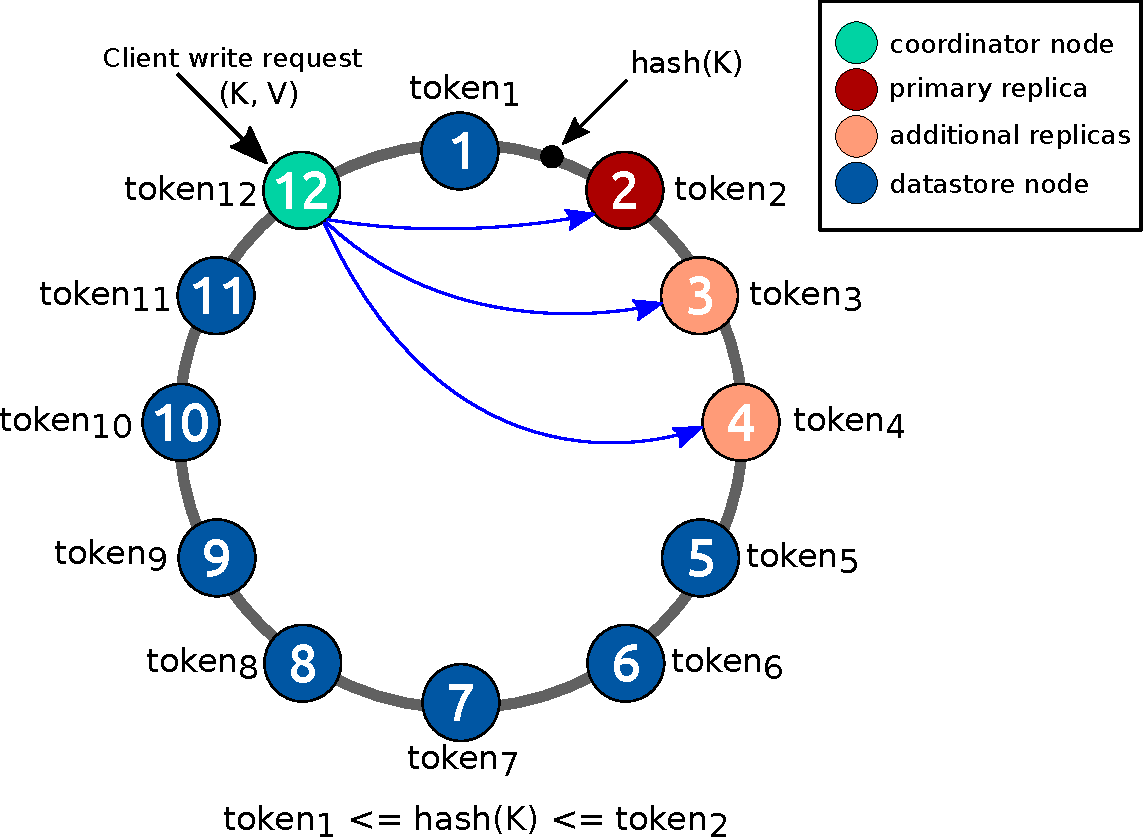
\includegraphics[width=0.7\linewidth]{figures/fogstore/basics/hashring.pdf}
\label{fig:hashring_replication}
\caption{Demonstration of write-request path for a 12-node
Cassandra cluster on keyspace with Replication Factor (RF)
= 3}
\end{figure}

\subsection{Control-plane Decisions involved in a Key-Value Store}
FogStore is a geo-distributed key-value store with data stored on multiple Edge sites. FogStore needs to make the following two control-plane decisions.
\begin{itemize}
\item \textbf{Replica Placement.} FogStore needs to determine the data store nodes that should host the replicas for a particular of data-item.
\item \textbf{Quorum Sizing. } For each query, FogStore needs to decide how many of the existing replicas of the queried data-item should be contacted before returning the result to the client. For read queries, the query coordinator node reads the data-item from Q replicas of the data-item and returns the latest version to the client, where Q denotes the quorum size selected. Similarly in the case of an insert or update query, the query coordinator returns success to the client as soon as the query has been executed on Q replicas.
\end{itemize}

\subsection{Application Requirements}
\begin{itemize}
\item \textbf{Low-Latency of Data Access. } State access is in the critical-path of typical applications. Hence, low-latency data access would allow the application instances to maintain their response-time.
\item \textbf{High Consistency. } For those data-items that have multiple readers and writers, applications require that the version of data that they read is the latest version. Reading a stale version of the data could result in errors in the application logic. Ensuring strong consistency in the application layer requires significant development time and often leads to complicated and error-prone mechanisms \cite{shute2013f1}. Hence, the data store is responsible for providing data access with strong consistency guarantee.
\item \textbf{Failure Tolerance. } Applications assume that with sufficient number of replicas of each data-items, at least one copy of a data-item will always be available for accessing in the event of failures.
\end{itemize}

\subsection{Challenges in achieving Application Requirements}
Operating a data store over a geo-distributed Edge infrastructure has a number of unique challenges arising out of the nature of the infrastructure.
\begin{itemize}
\item Network topology of the Edge infrastructure is heterogeneous, with Edge sites connected to the Internet through different peering points. This makes the latency between Edge sites heterogeneous. Hence, the data-placement strategies used in cloud-based data stores that ensure uniform load-balancing across storage nodes would result in high data-access latencies at the Edge.
\item High-consistency data read and writes require performing operations with multiple replicas of a data-item. In an Edge-based data store, where the inter-node latency distribution is heterogeneous, low-latency data access with high-consistency can only be achieved if all the replicas in the quorum are located close to the query coordinator.
\item Edge infrastructure consists of sites that often share the same network and power lines. These sites are susceptible to geographically correlated failures. Hence, placing all replicas of a data-item on nodes in proximity of each other to ensure low-latency high-consistency access would result in making that data-item more vulnerable to such failures. In such an event, all replicas of that data-item would be lost.
\item Data-items that compose the state of situation-awareness applications are generated due to activity in the physical environment. Spatial skews exist in the distribution of activity. For instance, within a city, there may be surveillance cameras deployed only in a certain portion of the city (e.g. Downtown), which would create a skew in terms of the number of events pertaining to those areas compared to rest of the city. Storing data-items on storage nodes that are located close to the location of the data-item itself would result in workload skews, which would impact query performance and increase the storage requirement on a subset of nodes. This problem is avoided in datacenter-based data stores by using consistent hashing \cite{consistent_hashing} to distribute data-items across storage nodes, but that would significantly deteriorate query latency in a geo-distributed data store.
\end{itemize}
Hence, low-latency, high-consistency and tolerance from geographically-correlated failures are conflicting objectives in an edge infrastructure setting.

\section{Architecture of FogStore}
\label{sec:fogstore_arch}
In this section, we first describe the edge-centric control-plane policies in FogStore at a high-level, that allow it to meet the application requirements. Then we discuss the functionalities of the system components in FogStore.

\subsection{Edge-centric Control-plane Policies}
FogStore's control-plane policies for replica placement and quorum sizing aim at simultaneously providing the application requirements of low-latency, high-consistency and tolerance from geographically-correlated failures, while dealing with the specific challenges of the Edge infrastructure. It does so by utilizing a peculiar characteristic in the data-access pattern of situation-awareness applications, wherein certain data-items are of higher relevance for the application logic if they are located in the \textit{spatial context} of a given instance of the application. We call the spatial context of the application instance Context of Interest, which is explained further in the following.
\subsubsection{Context of Interest}
Situation-awareness applications have a strong notion of locality-awareness. For example, in the case of publish-subscribe systems, the publishers and subscribers are often located geographically close to each other, because the events they are concerned with pertain to the local geographical area. This property was exploited by Teranishi et al. \cite{teranishi2015scalable} with the Locality-aware publish-subscribe system. In general, geo-distributed applications possess the notion of contextual relevance, in that a given data-item is more relevant in a certain context than another. The notion of context is highly application-specific. For instance, in the use-case mentioned in \cref{sec:fogstore_application}, a vehicle detection is relevant at a higher degree in a context around the event in space and time, that is, within 5 kms from the event’s location and within 10 minutes of the event generation. This is because of the nature of the application - to build an accurate trajectory of a vehicle, the previous detection has to be in proximity to the current detection. Similarly, smart cars accessing the state of a traffic light (red/green), where the cars located in proximity to the traffic light, would require consistent access to traffic light state to prevent collisions. Clients not in the traffic light's proximity would be able to live with data that may be stale, that is, eventual consistency may be good enough for them. Often the data generated by Internet-of-Things applications are used for big-data analysis, which are offline batch processing tasks and don’t require highly consistent data. In the context of key-value stores, the notion of relevance translates to consistency and staleness as follows : all relevant items must be available in a consistent manner with minimum staleness. In other words, for a data-item $I$ all entities for whom $I$ is contextually relevant must see updates to $I$ in the same order (serializability) and with as low staleness as possible (real-timeliness).

\par We now formally define the above notion of contextual relevance. Fogstore allows the application developer to specify a generic (possibly conservative) \emph{region of relevance} (also called Context of Interest) around each data item such that operations originating from that region are executed in a strongly consistent manner. In this paper, this region of relevance is articulated as a bounding box in geographical space. The size of the CoI is configurable and application-specific. Fogstore would compare the location of a client to the location of the queried data-item and would provide a strongly consistent result only when the client's location lies within the CoI of the data-item. Clients beyond the region of relevance are typically not using the data for critical operations and hence can tolerate inconsistent/stale data to the same extent as an eventually consistent database.

\subsubsection{Two Replica Types offering Differential Consistency}
\label{sec:two_replica_types}
We would like to revisit the two fundamental requirements of situation-awareness applications:
\begin{itemize}
\item Clients sharing context with the data-item require low-latency access to strongly consistent data
\item Placement of all replicas in proximity may lead to complete data loss under geographically-correlated failures
\end{itemize}

These requirements lead us the design decision of having two classes of replicas, which is also illustrated in \cref{fig:architecture}.
\begin{enumerate}
\item \textbf{In-CoI replicas} : Placed on nodes located at low network delay from the clients, typically within/around the CoI of the data-item.  Their maximum distance from the data-item's location is determined by a parameter \emph{InCoIDist}. This parameter determines the location of InCoI (strongly consistent) replicas and hence has implications on the latency of query operations. These replicas are kept consistent by enforcing that all read and write quorums include a majority of these replicas. These replicas are meant to provide both low-latency and strong-consistency to users that are contextually relevant to the queried data-item.
\item \textbf{Out-CoI replicas} : The purpose of these replicas is to provide tolerance from geographically-correlated failures. They are placed on datastore nodes which are a minimum distance away from the data-item's location, a parameter called \emph{OutCoIDist}. This parameter determines the location of OutCoI replicas, and hence affects the geographical separation between InCoI and OutCoI replicas - and thereby the fault-tolerance. These replicas are kept eventually consistent by propagating updates asynchronously, and hence are never included in the read/write quorum operations originating from within the CoI. These replicas could also serve as the source of data for big-data analysis of information generated at the edge, by using tools like Kafka Connect \cite{kafkaconnect} that can use key-value stores as data sources for large-scale analytics.
\end{enumerate}

\begin{figure}[h]
\centering
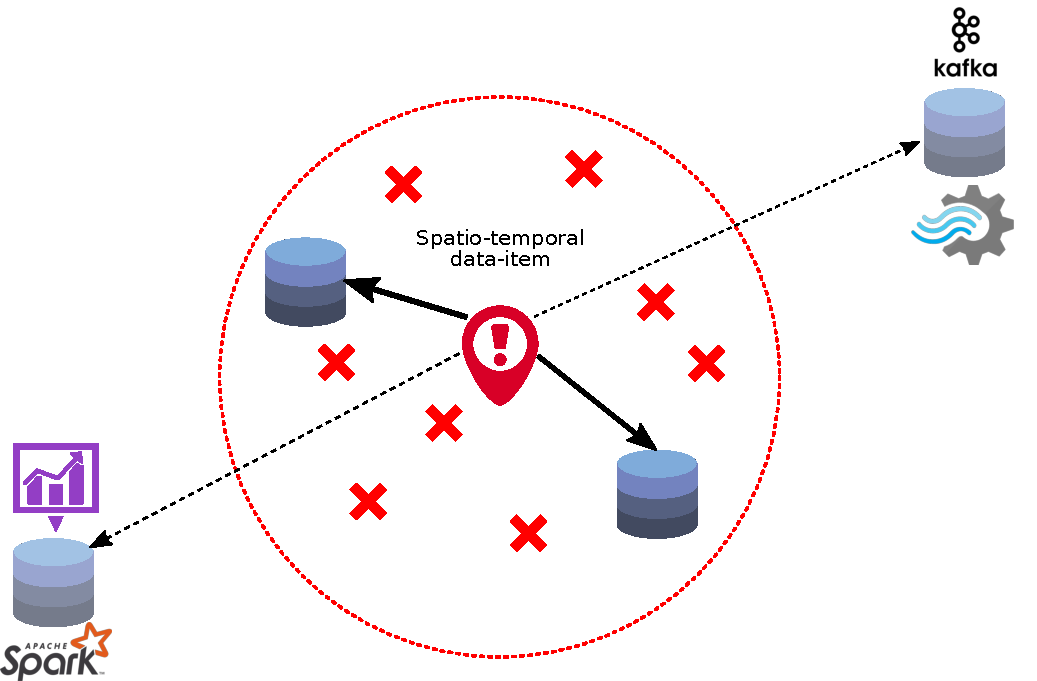
\includegraphics[width=0.8\columnwidth]{figures/fogstore/architecture.pdf}
\caption{Illustration of the two types of replicas maintained by Fogstore along with the typical use-cases that both these types serve. The dotted circle around the spatio-temporal data-item denotes the Context-of-Interest for the data-item. We direct all reads/updates to that data-item originating within the CoI (represented by red crosses) to the InCoI replicas (which are shown inside the circle). The other (OutCoI) replicas are kept eventually consistent and serve the use-cases dealing with batch processing and monitoring.}
\label{fig:architecture}
\end{figure}

\par It is worth noting that the concept of differential consistency for replicas based on their context is not a novel concept proposed in this dissertation. Apache Cassandra itself provides a consistency level called LOCAL$\_$QUORUM \cite{localquorum} that makes sure that any operation selects a quorum that consists of the quorum-set of replicas on the local datacenter on which the request-handler (coordinator) node is located. This is done to avoid the high latency of inter-datacenter traversal. The updates are propagated to rest of the replicas (in other datacenters) in an eventual manner. However, this concept is easy to adopt in the context of cloud-based data-stores, which have a well-defined notion of datacenters such that the network latency across datacenters is at least an order of magnitude higher than intra-datacenter latency. Data stores deployed on densely geo-distributed Edge infrastructures cannot make use of such a concept, especially when the concept of contextual locality is based on node location and geographical distance rather than simpler properties like a datacenter identifier or IP address subnet. 

\subsubsection{Handling skews in event workload}
FogStore's replica placement policy ensures that InCoI replicas are located close to the location of the data-item, while also ensuring that the workload across data-storage nodes is balanced. It does so by incorporating a hash-based replica placement approach akin to datacenter-based data stores into the location-based policy. More concretely, among the candidate nodes that fulfil the condition of InCoI replicas being close to the data-item's location, FogStore tries to use hashing to map the replica to candidate nodes. By doing so, FogStore not only achieves location-awareness but also ensures that the workload is evenly distributed among all candidate storage nodes. This notion of proximity is tunable, and can be set to match the degree of skew in workloads.

\par Hence the major issues that the implementation of Fogstore should resolve are :
\begin{itemize}
\item Placement of replicas based on the data-item's context, so as to have replicas both in proximity serving the queries from relevant clients within the CoI with low-latency and also at a significant geographical-separation from the CoI to provide tolerance from geo-correlated failures.
\item Providing a transparent consistency interface to clients by determining the per-query consistency level based on contextual information of the client and queried item. This tuning of consistency-level is done by choosing the quorum of replicas in a way so as to deliver strongly consistent information to relevant clients and possibly stale information to clients outside the context-of-interest.
\item Avoid the formation of hotspots in data-partitioning due to inherent skews in the input workload.
\end{itemize}

\subsection{FogStore Client}
The client of FogStore is an entity in some situation-awareness application that needs to read or update state. It could be an end-client, such as an application module running on an autonomous vehicle querying the status of a traffic light in vicinity, or a module running on an Edge site as described in \cref{sec:fogstore_application}. Since the client is a component of a situation-awareness application, it is associated with a certain spatial context. The client provides the current spatial context to FogStore along with the query request. FogStore system would determine if the current spatial context of the client overlaps with  the Context Of Interest of the data-item being queried to determine the appropriate consistency level for executing the query.

\subsection{FogStore Servers}
FogStore is composed of multiple geo-distributed servers which act as the interface between the clients and the stored data. These servers perform two main functionalities. Firstly, they act as Coordinators for query execution, wherein they perform  the entire execution of the query on behalf of the client. The coordinator checks the location of the client and the CoI of the data-item being requested to determine whether the data-item is contextually relevant to the client. As discussed in \cref{sec:two_replica_types}, if the client is contextually relevant the quorum set for this query is set to a majority of the InCoI replicas (strong consistency), otherwise the quorum is set to 1 (eventual consistency). In other words, the coordinator would return the query result to the client after a quorum of replicas have returned the result.
\par Second, FogStore servers act as Data Storage Nodes which host replicas of data-items and respond to queries from the coordinators. Each data storage node is responsible for a partition of the hash-space (as described in \cref{sec:replication}) based on its token. Since FogStore performs location-aware replica placement, the token of a data store node is derived from its location.

\section{Use of Spatial Context Management mechanism for Replica Placement}
\label{sec:replica_placement}
In this section, we show how the Spatial Context Management mechanism is used for selecting replica placement candidates for a data-item. As described in \cref{sec:replication}, in Dynamo-style data stores, each data-item is hashed to generate a scalar value which is used to select the right node to host its replica. In FogStore's case, since replica selection needs to be based on location, the location field of data-items and storage nodes need to be converted into a scalar value to serve as the hash lookup key and node token respectively. The key idea in FogStore's use of the Spatial Context Management mechanism to use the spatial partitioning created by the mechanism as a geo-index to encode location to a scalar value.

\subsection{Using Spatial Partitioning for Spatial Encoding of Geographical Locations}
\label{sec:geoindexing}

We partition the entire geographical space containing the application workload and data store nodes using the Spatial Context Management mechanism. The partitioning is then used to geo-index data-items and storage nodes. Each vertex of the KD-Tree in the proposed spatial partitioning is assigned a unique ID based on the area that it covers. The root of the tree covers the entire geographical area in question, while the size of the smallest tile or leaf vertex is determined by the height of the KD-Tree. \cref{fig:fogstore_kd_tree} illustrates such a KD-Tree of height 2. 
\begin{figure}[ht]
  \centering
  \begin{subfigure}[b]{0.45\linewidth}
    \centering
    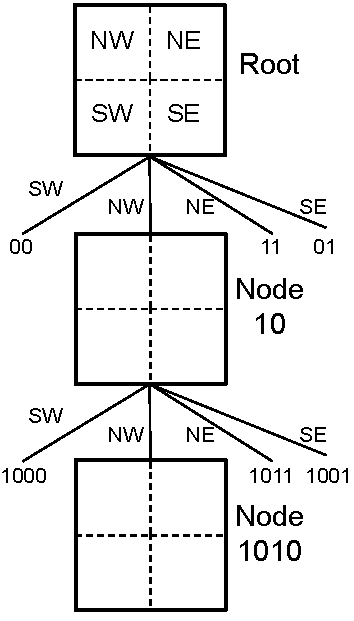
\includegraphics[width=0.75\linewidth]{figures/fogstore/kdtree.pdf}
    \caption{KD-Tree of height 2 for partitioning geographical space. Each node of the tree is split into 4 parts - Southwest (SW), Northwest (NW), Northeast (NE) and Southeast (SE). This figure only shows the Northwest child of each vertex.}
    \label{fig:fogstore_kd_tree}
  \end{subfigure}
  ~~~~
  \begin{subfigure}[b]{0.45\linewidth}
    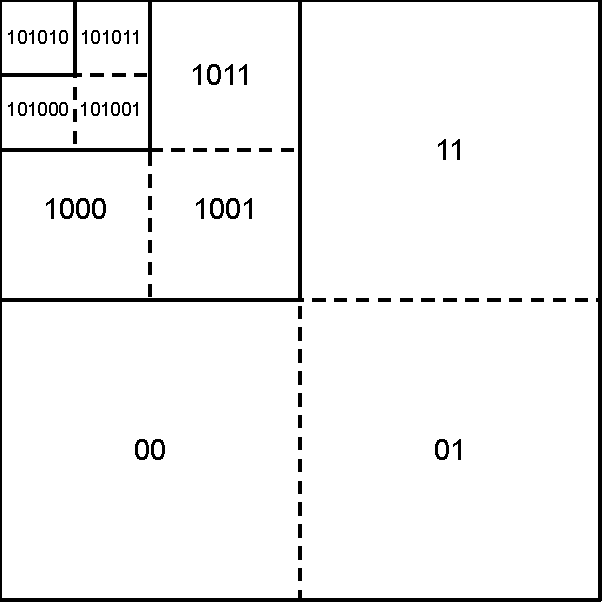
\includegraphics[width=\linewidth]{figures/fogstore/tile_ids.pdf}
    \caption{Spatial partitioning obtained by using a KD-Tree of height 3. As in \cref{fig:fogstore_kd_tree}, only the Northwest child of each vertex is expanded into its own children.}
    \label{fig:fogstore_tile_ids}
  \end{subfigure}
  \caption{Illustration of using KD-Tree based spatial partitioning in FogStore.}
  \label{fig:fogstore_partitioning}
\end{figure}
Each non-leaf node is partitioned the two axes - latitude and longitude - and therefore has 4 children. These children are termed as $child_{sw}$, $child_{nw}$, $child_{ne}$, $child_{se}$ respectively. \cref{fig:fogstore_tile_ids} illustrates how the ID of each child vertex can be derived from the ID of the parent vertex. We convert the ID of each node using base-32 encoding to a human-readable ID.
The height of the KD-Tree is configurable and can be tuned based on application-specific requirement of low-latency and uniform load balancing.
FogStore then encodes the location of a data-item or a storage node to the ID of the tile that the location maps to.

\par Each data-item has an additional field called $partition\_key$ which stores the ID of the leaf spatial partitioning tile that it belongs to. This ID forms the hash-value that is used to lookup the token ring for replicas. 

\subsection{Building the Token Ring}
\par In order to perform location-aware data distribution we use the spatial encoding (as described in \cref{sec:geoindexing}) of a data-item's location field to compose the partition-key. Datastore nodes are placed on the token-ring at a position equal to the spatial encoding of their location. In order to ensure that a data-item is placed on a node whose spatial-encoding is similar to the data-item's, it is important that tokens be ordered with respect to their spatial encodings for replica selection. Hence we don't use the popular consistent hashing algorithm for generating the token, but rather use the partition key directly as the token. 

\subsubsection{Notion of distance in spatial encoding}
\par We define a notion of distance between two spatial encodings which is core to choosing the right nodes to place replicas on. Two spatial codes $d1$ and $d2$, have a distance of $d$ if and only if $d1$ and $d2$ have the $d^{th}$ bit as the maximally significant bit that differs in them. This is clarified in \cref{fig:geohashdist}. This notion of distance can be applied to any spatial encoding technique used to calculate tokens. It preserves the closeness of locations, that is, if two locations are closeby in terms of the proposed encoding distance, they are also closeby in terms of geographical distance. The converse, however, is not true, that is locations that are close in geographical distance may have spatial encodings that are far apart in terms of encoding distance. This property is evaluated in \cref{sec:evals} when determining the location of OutCoI replicas \todo{Check if this evaluation is covered}.
\begin{figure}
\centering
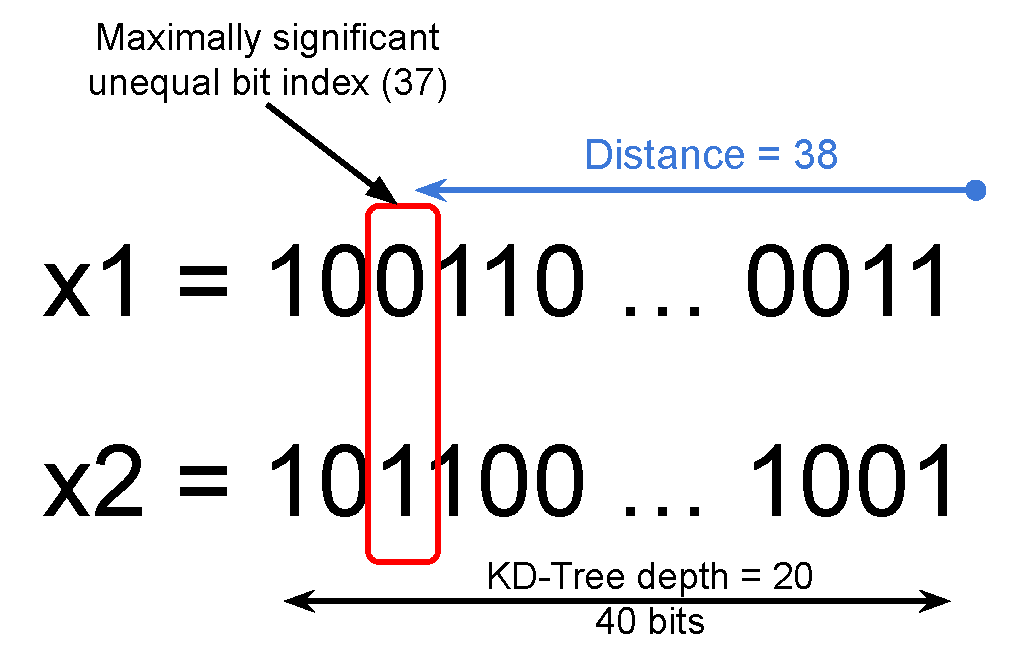
\includegraphics[width=0.8\columnwidth]{figures/fogstore/coi_distance.pdf}
\caption{An illustration of distance between the IDs of two tiles in a KD-Tree of height 20.}
\label{fig:geohashdist}
\end{figure}

\subsection{Selecting Candidate Replica Nodes based on Data Item's Spatial Context}
Selection of replicas for a given data-item is done based on the spatial encoding distance of a node's token and the data-item's token. The replica selection alogrithm takes the following two parameters :
\begin{itemize}
\item \emph{InCoIDist} : the maximum spatial encoding distance threshold for placing InCoI replicas. 
\item \emph{OutCoIDist} : the minimum spatial encoding distance threshold for placing OutCoI replicas.  
\end{itemize}

The first node token that the item's token gets mapped to in the token ring is used as the starting point for iteration to find the InCoI replicas. Each potential node that is within CoI's distance threshold is a suitable candidate. A similar search is performed for getting the list of OutCoI replicas, the difference being that the spatial encoding distance between item's token and node's token now needs to be greater than the CoI distance threshold.

\subsection{Ensuring Even Load Distribution among Data Storage Nodes}
\par The distribution of spatio-temporal event traffic is not expected to be uniform, with much more activity in densely populated regions and lesser activity in sparsely populated regions. Forming a node's token solely based on the spatial encoding would lead to partitions in the hash ring not being uniform in the number of tokens contained in them. This can lead to uneven distribution (poor load balancing) of key-value pairs across data store nodes. Consistent hashing forms one extreme of data partitioning that achieves best load balancing, but does not take into account spatial locality of replicas, while just using spatial encoding forms the other extreme which guarantees spatial locality but not load balancing.
Hence, the two objectives of proximal data placement and load balancing prompts us to come up with a hybrid data partitioning scheme. We construct the partition-key $PK$ of a data-item $i$ as shown in Figure \ref{fig:partitionkey}.
\begin{figure}[h]
\centering
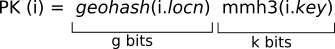
\includegraphics[width=0.75\columnwidth]{figures/fogstore/partitionkey.png}
\caption{Illustration showing the inclusion of location-specific information in data-item's token to enforce proximal placement and the hash of key for even distribution.}
\label{fig:partitionkey}
\end{figure}

\subsection{Replica Placement Algorithm}
The replica selection policy for InCoI replicas is presented in Algorithm 2. The first node token that the item's token gets mapped to in the token ring is used as the starting point for iteration to find the InCoI replicas. Each potential node that is within CoI's distance threshold  and has a token with key portion lexicographically higher than item's token is a suitable candidate. Note that the comparison of token's key portion is solely for load balancing purposes. A fixed number of such replicas are selected. If the required number of replicas are not found after a complete traversal of the ring, the CoI's distance threshold is incremented by a small amount and the search is repeated. This increase in the threshold (which is specified by application developer) may harm the expected latency, but we choose to do so over declaring that no suitable replicas could be found.
\begin{algorithm}
\caption{Replica selection algorithm}\label{incoireplicaselection}
\begin{algorithmic}[1]
\Procedure{findPrimaryReplica}{$H, itemToken, it_S$}
\State $it_P \gets $ null
\For{$it \in iterate(H, it_S)$}
	\If {$ itemToken \leq it \& it.key \geq itemToken.key$}
		\State $it_P \gets it$
		\State $break$
	\EndIf
\EndFor
\If {$it_P == $null}
	\State $it_P \gets it_S$
\EndIf
\Return $it_P$
\EndProcedure
\Procedure{findReplicas}{$H, itemToken, it_P, inCoiDist, N$}
\State $replicas \gets \{\}$
\For{$it \in iterate(H, it_S)$}
	\If{$geohashDist (it.geohash, itemToken.geohash) \leq inCoiDist \quad \& \quad it.key \geq itemToken.key \quad \& \quad it \text{ not already chosen}$}
		\State $replicas = replicas \cup \left\{ {it} \right\}$
	\EndIf
	\If{$\left\vert{replicas}\right\vert == N$}
		\State $break$
	\EndIf
\EndFor
\Return $replicas$
\EndProcedure
\Procedure{findInCoIReplicas}{$H, itemToken, inCoiDist, nReplicas$}
\State $it_S \gets H.find(itemToken)$
\State $it_P \gets findPrimaryReplica (H, itemToken, it_S)$
\State $nFound \gets 0$
\State $inCoiReplicas \gets \{\}$
\While{$\left\vert{inCoiReplicas}\right\vert < nReplicas$}
	\State $R \gets findReplicas(H, itemToken, it_P, inCoiDist, nReplicas-nFound)$
	\State $inCoiReplicas \gets inCoiReplicas \cup R$
	\State $nFound \gets nFound + \left\vert{R}\right\vert$
	\State $inCoiDist++$
\EndWhile
\Return $inCoiReplicas$
\EndProcedure
\end{algorithmic}
\end{algorithm}

\section{Use of Spatial Context Management mechanism for Consistency Tuning}
\label{sec:consistency_tuning}

Selection of replicas constituting a quorum based on the context of interest of data item queried for is done based on the token of the coordinator node \footnote{The underlying assumption is that client and coordinator node are in relative proximity}. We use a parameter \emph{CoISize}, which represents the size of the CoI in terms of spatial encoding distance.  If the coordinator's token is less than \emph{CoISize} units distant from the item's token, it lies within the CoI of the queried data item, and a quorum of InCoI replicas are selected to sychronously execute the operation. This ensures that all operations within the CoI will be highly consistent. Read operations on coordinators that are outside the CoI of queried data item are returned the version from whichever replica responds the fastest, thus providing eventual consistency. Write operations, on the other hand, need to update a quorum of the InCoI replicas before returning so that InCoI replicas don't enter an inconsistent state. Enforcing quorum for operations inside the CoI is fast as the quorum members are located in close network proximity from the client/coordinator node.

\subsection{Optimizations for efficient range queries}
\todo{Remove reference to Cassandra} Typical deployments of Cassandra key-value store use consistent hashing (Murmur3 hash) on the partition-key to partition the key-value pairs across nodes. Since the Murmur3 hash function does not preserve the order between input values, Cassandra does not allow range queries on the partition key. However, Fogstore uses the ByteOrderedPartitioner which preserves the order between partition-keys, thus making it possible to issue range queries on them. A typical range query has a structure as shown in Listing \ref{lst:rangequery}.
\begin{lstlisting}[caption={Typical form of a range query that Fogstore handles. The minimum and maximum limits of partition key range queried for is calculated based on the bounding-box of locations that forms the range query. Note that we omit timestamp based filtering for simplicity, however that can be incorporated in the query provided a secondary index is built on the timestamp field.},captionpos=b,label={lst:rangequery},language=SQL]
SELECT * FROM tracking_ks.detections 
WHERE token(part_key)>=token(<min_part_key>) AND 
token(part_key)<=token(<max_part_key>) AND 
key='<object_key>' 
\end{lstlisting}
\par For efficient execution of this query, a secondary index on the $key$ column is created so that events within a particular partition can be queried in lesser time. Upon receiving such a query, the coordinator node splits the range into individual partitions and issues concurrent read requests to the replicas responsible for those partitions. 

\section{Evaluations}
\label{sec:evals}
We implement the architecture present above by extending Apache Cassandra. We use the distributed network emulator MaxiNet \cite{maxinet} to create the infrastructure setup for evaluation experiments. MaxiNet is an extension of the popular network emulator MiniNet, and allows the user to package an application as a Docker container and deploy it on a set of nodes. Latencies between the nodes are calculated using the geographical distance between the nodes based on the online tool WAN Latency Estimator\footnote{http://wintelguy.com/wanlat.html}.

\begin{figure}[h]
\centering
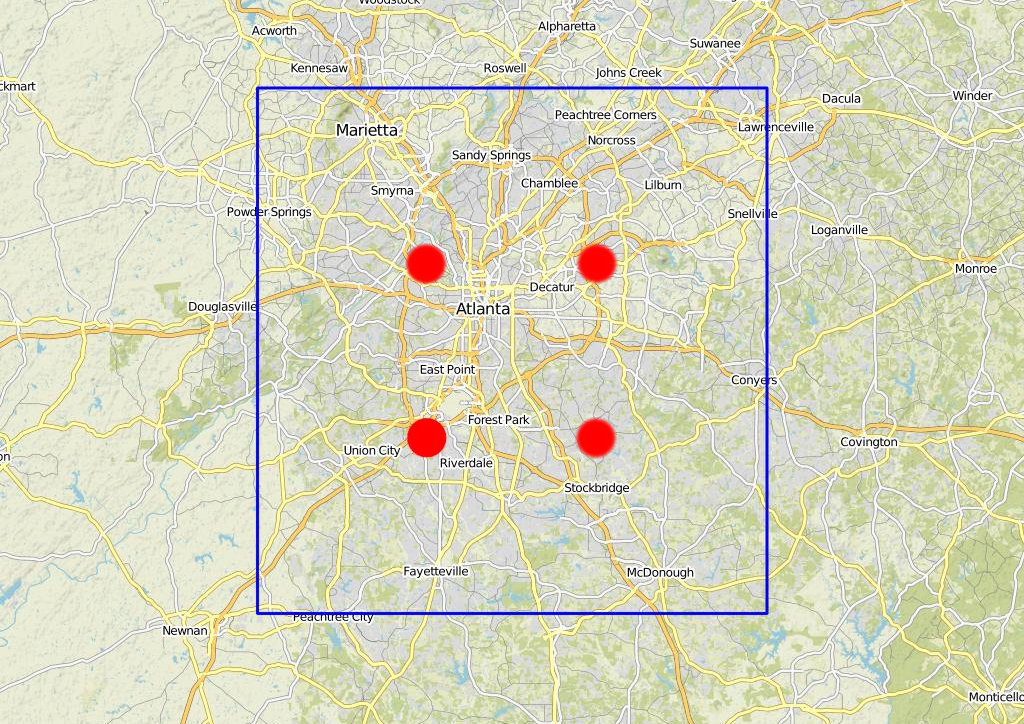
\includegraphics[width=8cm]{figures/fogstore/evals/hotspot/map-cropped.jpg}
\caption{Map showing the locations of fog nodes in Atlanta region and the bounding box from where events are generated. The nodes shown in the figure are the ones that store the InCoI (consistent) replicas in Fogstore. The evaluation also consists of nodes located at remote locations : Houston, San Francisco, Chicago and Seattle.}
\label{fig:hotspotmap}
\end{figure}

\subsection{Comparison of FogStore against typical replication policies}
The first step towards proving the efficacy of the context-aware policies of Fogstore is to evaluate its performance against typical replication policies - quorum-based (strict) and eventual\footnote{The strict and eventual systems use Cassandra's SimpleStrategy policy for replication.}. 
%The aim of these experiments is to show that Fogstore provides consistency upto the level of quorum-based replication and throughput of the likes of eventual consistency. 
For this experiment, we build a representative infrastructure topology of datastore nodes - 4 inside Atlanta region and 4 more as remote datacenters. Yahoo Cloud Serving Benchmark (YCSB) is used to generate spatio-temporal workloads of applications running in the Atlanta area, by having 4 client nodes running YCSB with 4 threads each. Each YCSB client is collocated with one of the datastore nodes in Atlanta area and mimics a situation-awareness application component making queries to the spatio-temporal state. To cover a wide variety of workloads, we experiments with workloads that have varying read-to-update ratios (20\%, 50\% and 80\% reads) and varying distribution of selecting keys for operations (hotspot, latest and Zipfian). We consider mutable data-items to measure the behaviour of evaluated systems on consistency. We set the replication factor of eventually consistent and quorum-based store to 3. For the replication policy of Fogstore, we set number of InCoI replicas to 2 and OutCoI replicas to 1. Also, the read and write quorum for queries by clients inside the CoI are set to 2 and 1 respectively. 

\par To be able to perform these experiments and collect the required metrics, we had to modify the core workload executor of YCSB. Here we describe the major modifications to YCSB here :
\begin{itemize}
\item We associate each version of an entity with a given key with a timestamp, which corresponds to the wall-clock time when the YCSB client starts updating or inserting that version. When updating the entry in the table, we also add the timestamp associated with that version to that entry. We also record the time when an update/insert finishes. Since the experiment is done as an emulation on a single machine, the clocks of all datastore nodes and YCSB clients (Docker containers) use the time of the underlying physical machine.
\item We associate each key generated by YCSB to a unique geolocation, since the spatial attributes of a data-item is central to the consistency model of Fogstore. The challenge here is to create a deterministic mapping between the key domain and the geolocation domain - so that this mapping stays the same across all the threads on all YCSB clients. Each key selected by the request distribution of YCSB is based on an integer value, which we convert to a sequence of bits. This bit sequence is then decoded (exactly same as Geohash decoding) to generate the latitude and longitude of the request.
\item We needed to modify Python's driver for Cassandra to allow queries to have CoI-aware consistency level.
\item We use the latency aware load balancing policy to avoid choosing a coordinator that is too far away in terms of network latency - effectively defeating the purpose of Fogstore.
\end{itemize}

\par The metrics we are interested in are :
\begin{itemize}
\item Latency of read/update operations
\item Throughput of read/update operations
\item Client-centric degree of consistency
%\item Data-centric degrees of consistency
\end{itemize}

\begin{figure*}[t]
  \centering
  \begin{subfigure}[b]{0.32\linewidth}
    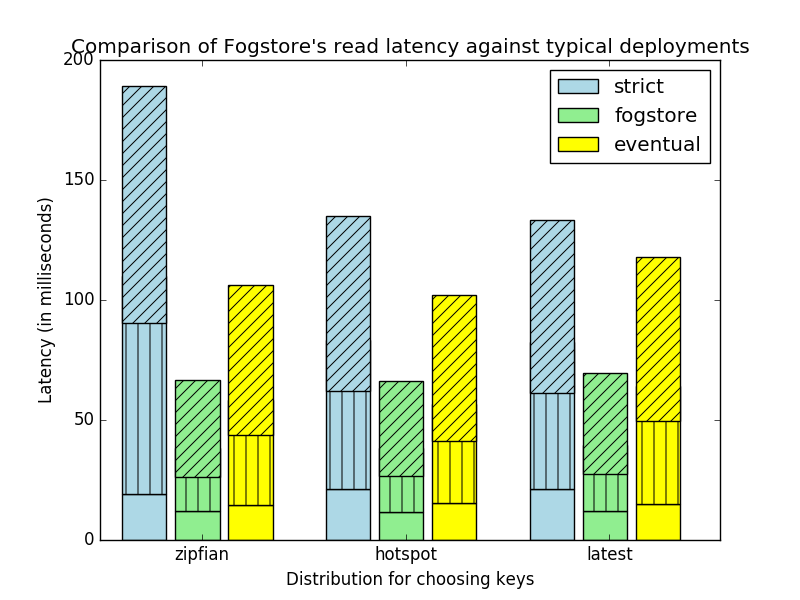
\includegraphics[width=\linewidth]{figures/fogstore/evals/stress-tests/0.2/read.png}
    \caption{20\% reads}
  \end{subfigure}
  \begin{subfigure}[b]{0.32\linewidth}
    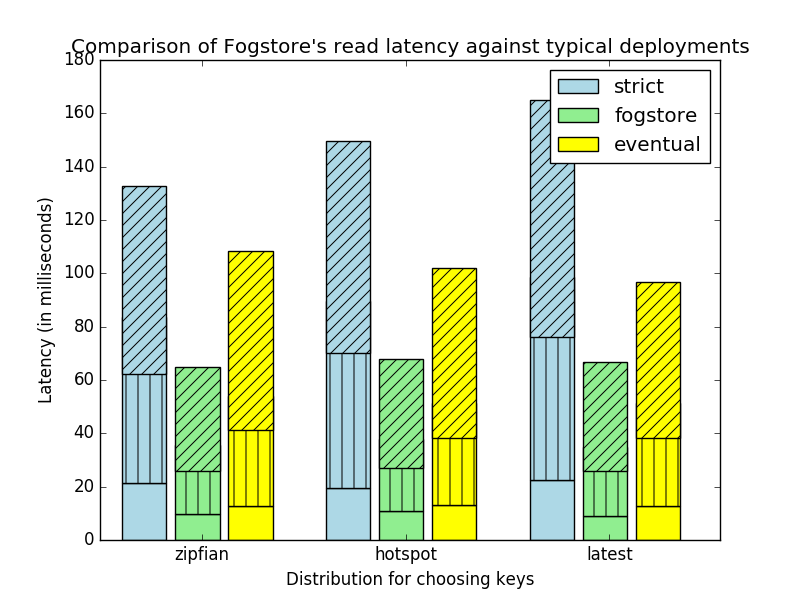
\includegraphics[width=\linewidth]{figures/fogstore/evals/stress-tests/0.5/read.png}
    \caption{50\% reads}
  \end{subfigure}
  \begin{subfigure}[b]{0.32\linewidth}
    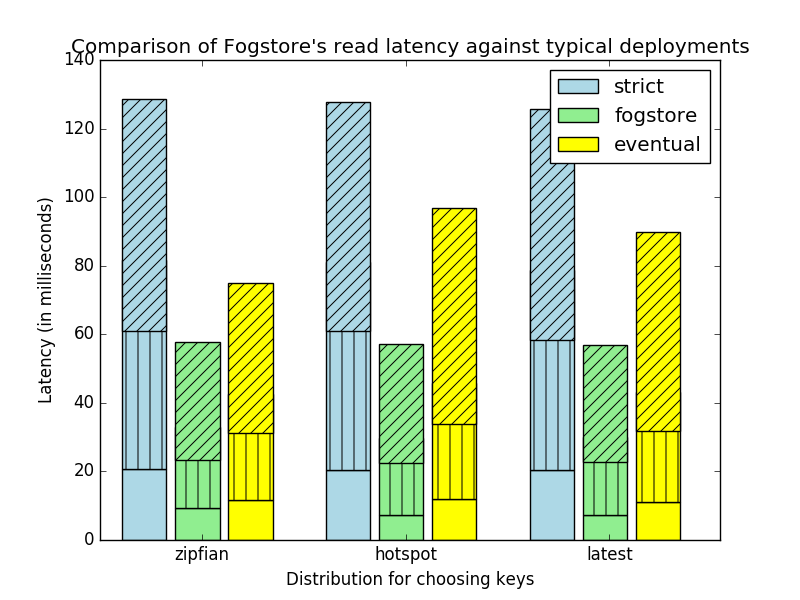
\includegraphics[width=\linewidth]{figures/fogstore/evals/stress-tests/0.8/read.png}
    \caption{80\% reads}
  \end{subfigure}
  \caption{Read latencies for varying distribution of reads. The solid, vertically dashed and obliquely dashed portions of the bar denote $50^{th}$, $95^{th}$ and $99^{th}$ percentiles respectively.}
  \label{fig:read-latencies}
\end{figure*}

\begin{figure*}[t]
  \centering
  \begin{subfigure}[b]{0.32\linewidth}
    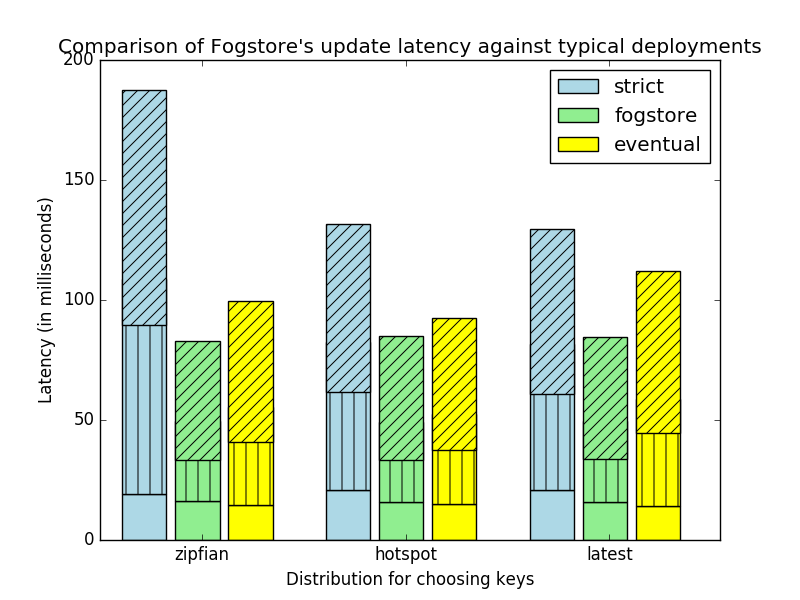
\includegraphics[width=\linewidth]{figures/fogstore/evals/stress-tests/0.2/update.png}
    \caption{20\% reads}
  \end{subfigure}
  \begin{subfigure}[b]{0.32\linewidth}
    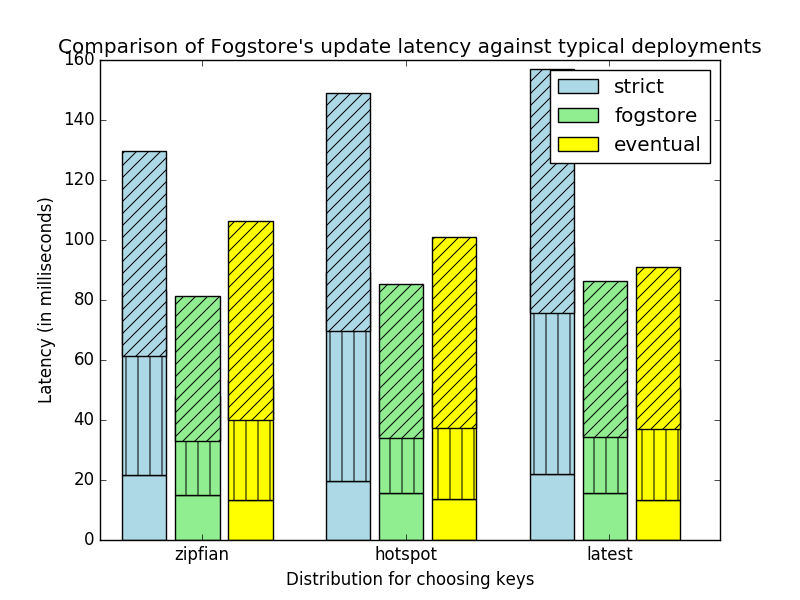
\includegraphics[width=\linewidth]{figures/fogstore/evals/stress-tests/0.5/update.png}
    \caption{50\% reads}
  \end{subfigure}
  \begin{subfigure}[b]{0.32\linewidth}
    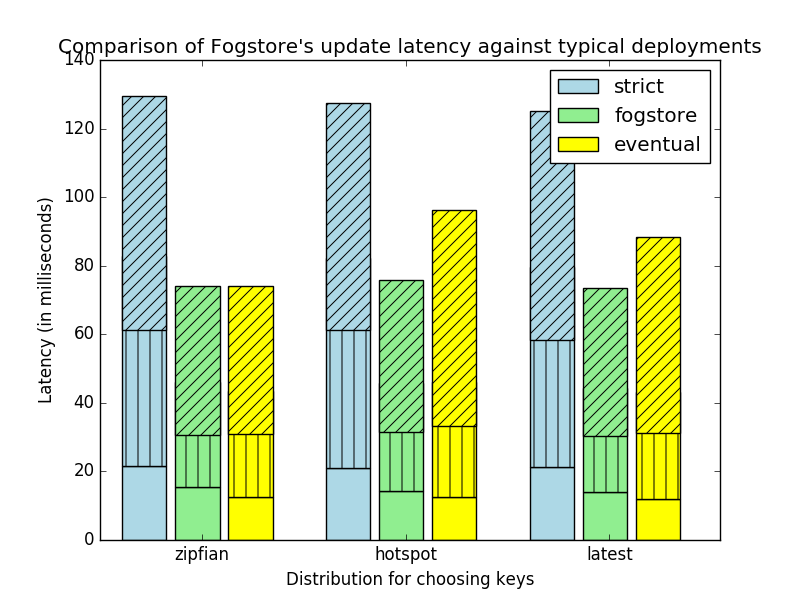
\includegraphics[width=\linewidth]{figures/fogstore/evals/stress-tests/0.8/update.png}
    \caption{80\% reads}
  \end{subfigure}
  \caption{Update latencies for varying distribution of reads. The remaining operations are updates. The solid, vertically dashed and obliquely dashed portions of the bar denote $50^{th}$, $95^{th}$ and $99^{th}$ percentiles respectively.}
  \label{fig:update-latencies}
\end{figure*}

\begin{figure*}[t]
  \centering
  \begin{subfigure}[b]{0.32\linewidth}
    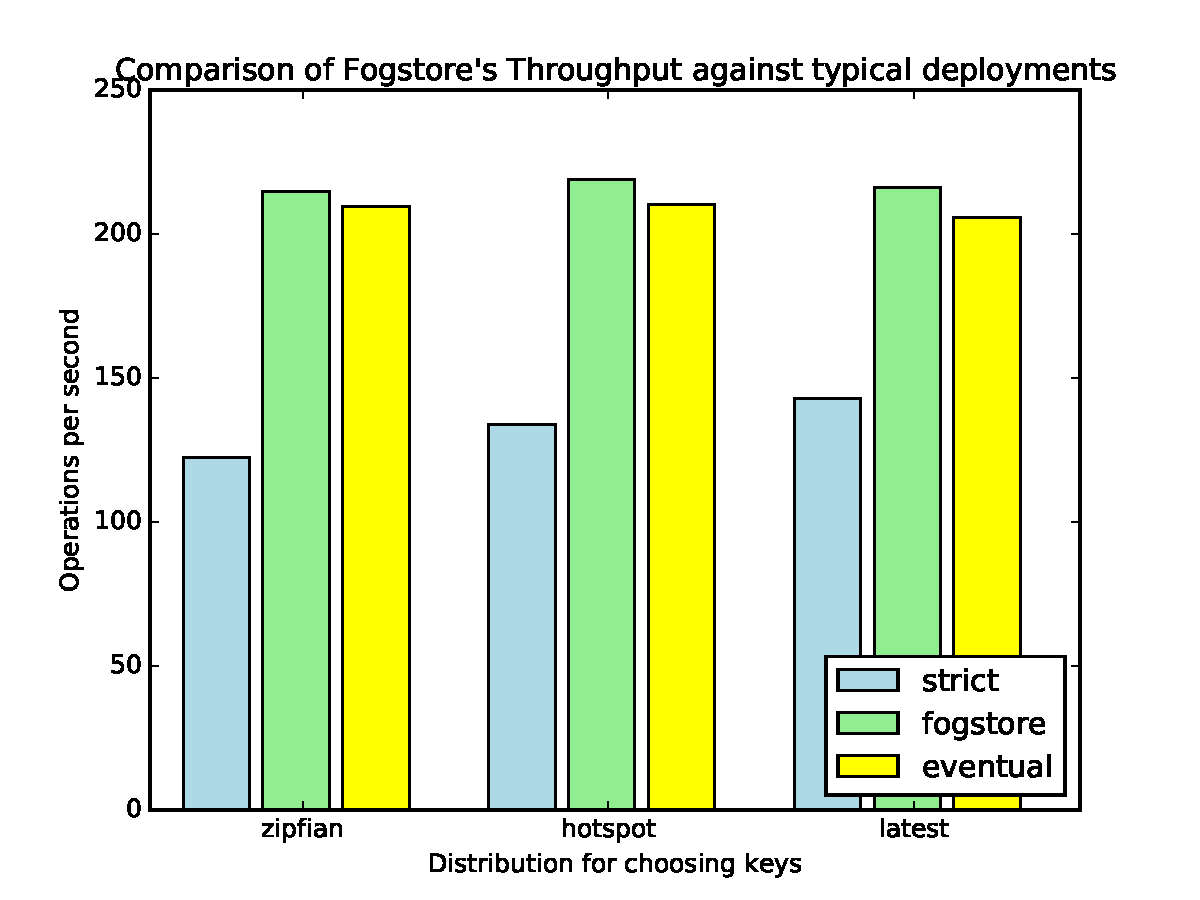
\includegraphics[width=\linewidth]{figures/fogstore/evals/stress-tests/0.2/tmp.pdf}
    \caption{20\% reads}
  \end{subfigure}
  \begin{subfigure}[b]{0.32\linewidth}
    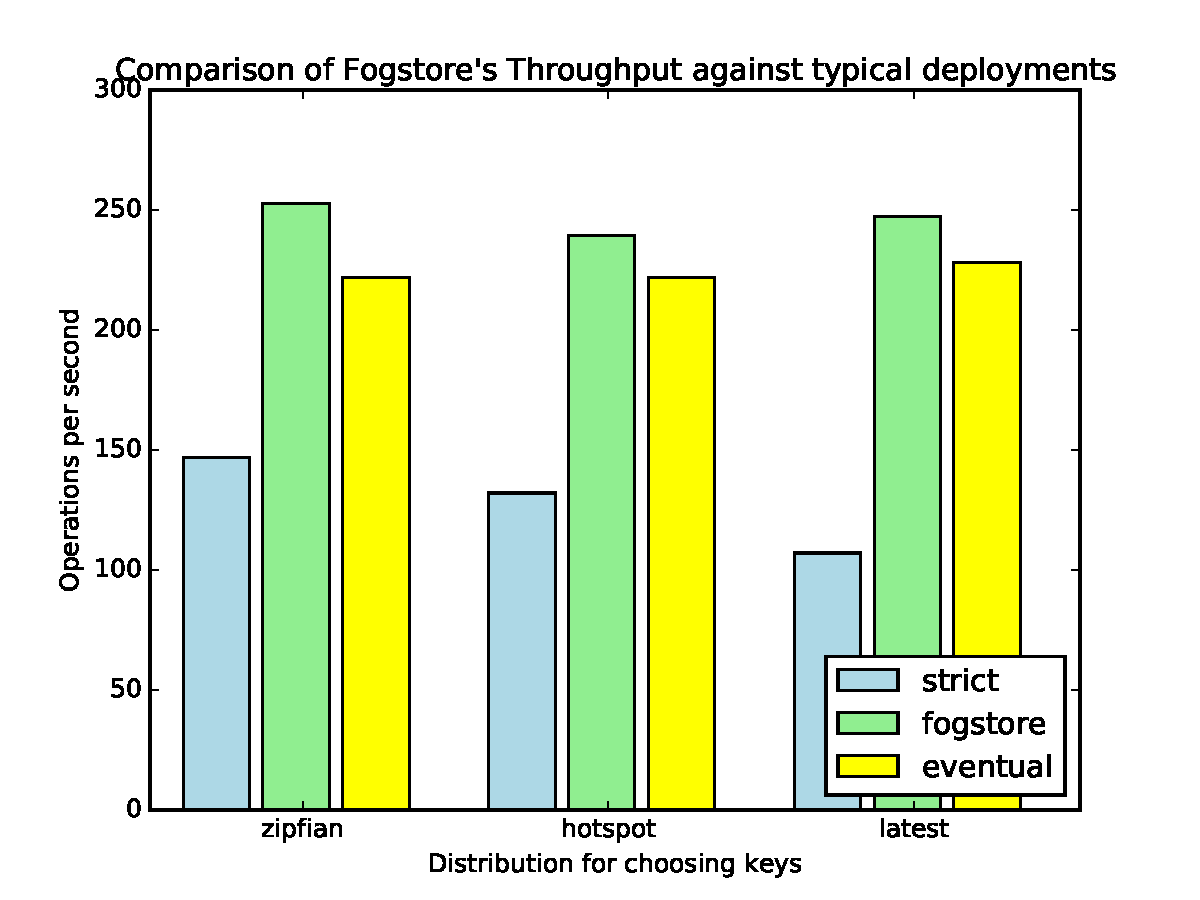
\includegraphics[width=\linewidth]{figures/fogstore/evals/stress-tests/0.5/tmp.pdf}
    \caption{50\% reads}
  \end{subfigure}
  \begin{subfigure}[b]{0.32\linewidth}
    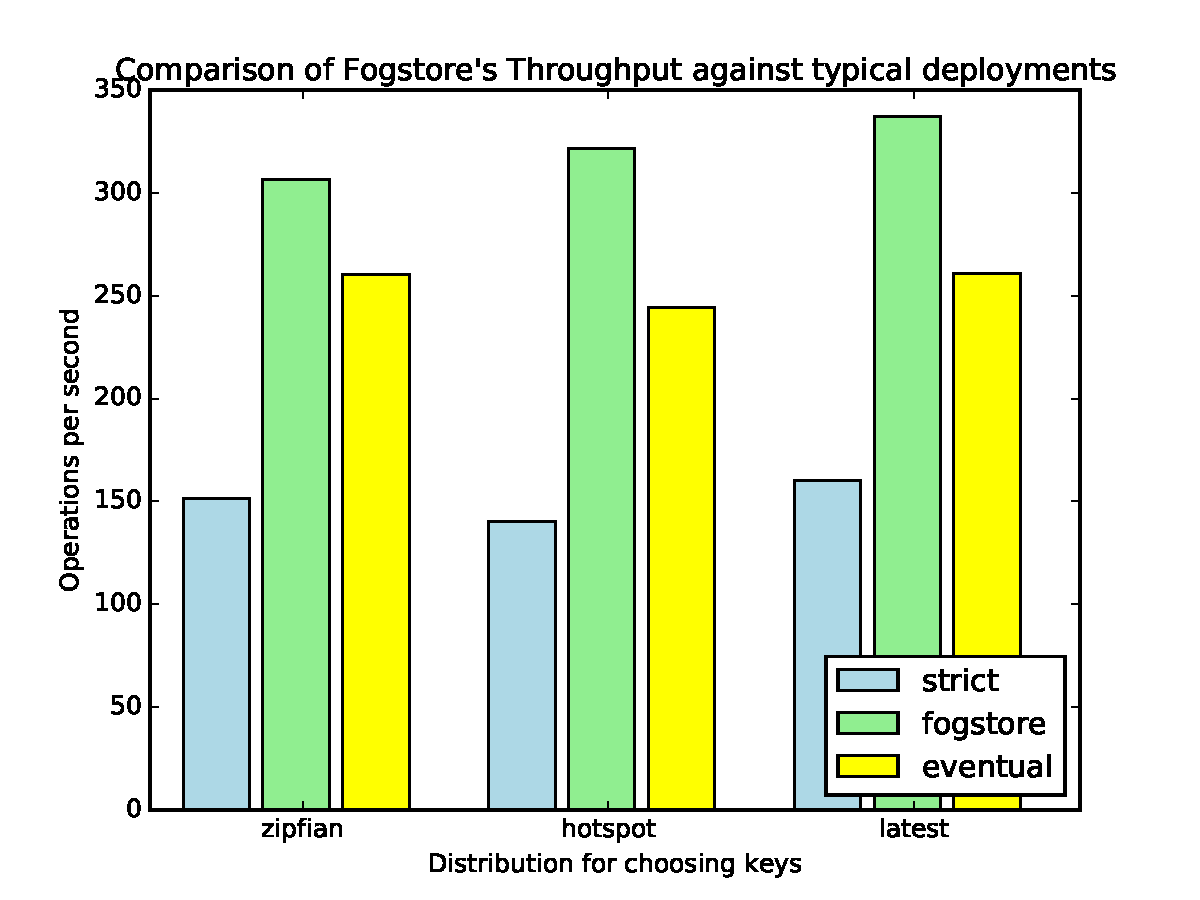
\includegraphics[width=\linewidth]{figures/fogstore/evals/stress-tests/0.8/tmp.pdf}
    \caption{80\% reads}
  \end{subfigure}
  \caption{Throughput (ops/sec) for varying distribution of reads}
  \label{fig:tputs}
\end{figure*}

\par Applications that require strong consistency for data-accesses would use the aforementioned quorum-based (strict) datastore. The client's expectation from a datastore guaranteeing strong consistency is that a read always returns the most recent version whose update was successful. We analyze the trace of YCSB clients and for every read compare the version returned to the version that was written by the most recent successful update, and call it a violation if these versions don't match. We analyze the YCSB client trace against a quorum-based store and, following the expectation, don't find any violations as the read and write quorums overlap. This means that the application does not have to implement special logic for handling inconsistent/stale data reads.
\begin{table}
\centering
\begin{tabular}{ |c|c|c|c| } 
 \hline
 & 20\% reads & 50\% reads & 80\% reads \\ 
 \hline
 Latest & 0.17 & 0.6 & 0.11 \\ 
 \hline
 Hotspot & 0.06 & 0.06 & 0.02 \\ 
 \hline
 Zipfian & 0.03 & 0.02 & 0.01 \\ 
 \hline
\end{tabular}
\caption{Percentage of reads returning a version that was not most recently written.  The percentage of inconsistent reads has been reported for workloads with varying proportion of read requests and key-selection distribution.}\label{tab:consistency_violations}
\end{table}
\par This reduction in programming effort due to strong consistency guarantees from the datastore comes at a price on performance, as now each operation has to wait to complete on a quorum of nodes, which may have high network latency between them. This hypothesis is validated by the variation of read and update latencies shown in Figures \ref{fig:read-latencies} and \ref{fig:update-latencies} and the aggregate operation throughput shown in Figure \ref{fig:tputs}. The applications in this paper's context are heavily dependent on the low-latency execution of read and update operations, and hence guaranteeing performance of paramount importance. 
\par For the sake of performance, the applications at hand would use an eventually consistent datastore, and wait for each operation to complete on only one replica before acknowledging the user. The experimental results show that the eventually consistent datastore is able to outperform the quorum-based store significantly in terms of operation latencies and throughput (Figures \ref{fig:read-latencies}, \ref{fig:update-latencies} and \ref{fig:tputs}). However, since clients may initiate reads before previous updates to those data-items have been propagated to all replicas, there are mismatches between the version returned by read operations and the most recently written version. Table \ref{tab:consistency_violations} shows the percentage of reads that undergo such consistency violations. Note that due to the limitations of the emulation platform, we only have 16 client threads in these experiments, and increasing the concurrency would lead to more reads that violate strong consistency. Hence the improvement in performance comes at the cost of programming effort to handle inconsistent reads from the datastore. 
\par To counter the performance limitations of quorum-based and consistency violations of an eventually consistent  datastore, we run the same client workloads against Fogstore, which is fundamentally Cassandra extended with the context-aware policies for replication and quorum selection. Since the read and write quorums are limited to replicas placed close to the data-item and overlap, there are no consistency violations i.e., it offers strong consistency. On the performance side, we observe that read and update latencies are even better than that of the eventually consistent store. We reason that this is because of the location-agnostic replica placement in plain Cassandra, where all the 3 replicas of a data-item may be located on remote nodes, leading to high operation latency even with eventual consistency. Fogstore is, therefore, able to achieve a better throughput than the eventual store. In fact, since the read quorum is set to 1 and write quorum to 2, the throughput for a read-heavy workload beats the eventual datastore by a higher margin as the number of replicas to block for is just one.

\par Hence, based on these results, the context-aware optimizations of Fogstore allow it to obtain the performance of an eventually-consistent store and, at the same time, provide consistency guarantees similar to a quorum-based database. This enables the design of systems that are dependent both on high throughput and low programming effort of dealing with inconsistent operation results.

\subsection{Performance of range queries}
Applications processing spatio-temporal data have a high performance dependence on efficiency of range-queries. Fogstore performs data-distribution based on location, which would lead range queries to span across a number of datastore nodes. In the following set of experiments we analyze the performance of Fogstore for delivering results of range queries and the impact of range filter size. We compare the performance of range queries on Fogstore against a baseline eventually consistent database setup - which uses the data-item's \emph{type} to partition items across datastore nodes. Since events are not mutable, we are not dependent on consistency guarantees.
\par For this paper, we assume that range queries request events of a certain type $T$ in a circular geographical area of radius $R$ km centered at location $L$ and can be expressed as the tuple $(L, R, T)$. To support efficient range queries, we built a wrapper that transforms the tuple $(L, R, T)$ into a number of contiguous subset of geohashes, such that they cover the area covered by the range (similar to \cite{spatialcassandra}). For each of these subsets we trigger a \emph{child} concurrent sub-query to Fogstore that returns events with a location falling under the subset of geohashes. The range query is said to be completed when all the \emph{children} sub-queries are complete. For this set of experiments, we build a datastore cluster same as the previous experiment, with 4 nodes around Atlanta and 4 at remote locations (see Figure \ref{fig:hotspotmap}). A precision of 4 is chosen for encoding locations into Geohash, both for data-nodes' tokens and partition-key of data-items. We load the database with 4000 events of 10 different types from the area marked by the blue outline. For each range query $(L, R, T)$, $L$ is sampled from the bounding box in Figure \ref{fig:hotspotmap} while $T$ is sampled from the set of 10 event types. The value of $R$ is varied and the impact of its variation on range query completion time is reported in Figure \ref{fig:scan}. 
\begin{figure}[h]
\centering
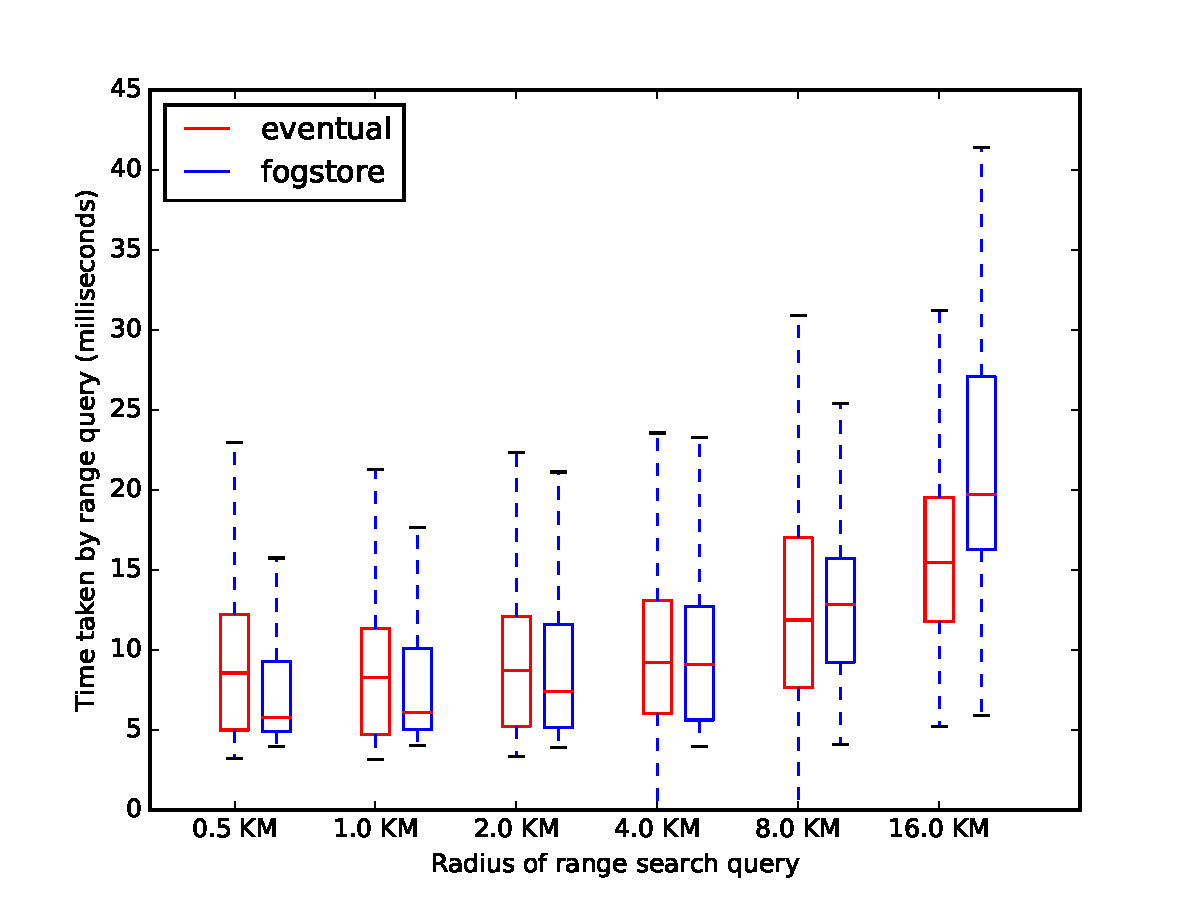
\includegraphics[width=0.75\columnwidth]{figures/fogstore/evals/scan/compWithEventual.pdf}
\caption{Comparison of latency of range queries with varying range-radius for Fogstore's data partitioning and eventually consistent Cassandra deployment. All statistics are aggregated over 5000 range queries.}
\label{fig:scan}
\end{figure}
\par As is evident from Figure \ref{fig:scan}, the location-based distribution of data done by Fogstore is able to achieve comparable performance to the baseline eventually consistent datastore with the increase in radius of range queries. Increasing the range-query radius increases the number of replicas (datastore nodes) that would store the events queried for, which increases the overhead on Fogstore's coordinator node to split the original sub-query further down into read requests that are sent to individual replicas. This factor, however, does not impact the baseline datastore, since the events are partitioned based on the item type field, which is fixed for a particular range-query, meaning each replica assigned to that item type would have all the data-items of that type. Furthermore, an increase in range-query radius also leads to increase in the number of events returned, which also impacts query-completion time, both for Fogstore and the baseline.

\subsection{Load balancing across data-store nodes}
One of the supposed limitations of partitioning data-items based on spatial encoding using Cassandra's hash ring mechanism is that skews in application workload can lead to some datastore nodes storing significantly more data-items than others. This is because of the fact that we want to preserve spatial proximity of replica placement. 

\par In order to perform large-scale tests of load balancing, we design a simulation environment which mimics the replica placement approach of Fogstore \footnote{The emulation platform used in previous experiments is not large enough to emulate a very large number of nodes}. We focus on the region around Atlanta, as shown in Figure \ref{fig:hotspotmap}, and place 64 datastore nodes within that region in a uniformly-spaced manner. To simulate spatial skew in data access pattern, we generate 80\% of the data-items from a small area (0.0625 times the full region) around Downtown while the rest of the region generates 20\% of data-items. For every data-item we set the number of InCoI replicas to 2, and configure the CoI distance so as to have all the 64 fog nodes candidates for hosting the InCoI replicas. Furthermore, we also envision having multiple datastore nodes deployed at a particular resource location, akin to a mini-datacenter. The data-partitioning policy should be able to utilize all the available capacity, both at the same location as well as across multiple locations. The metric of interest is the number of data-items that each node is assigned. A data partitioning policy that does not take load-balancing into account would lead to nodes close to the hotspot region storing much more data-items than those away from it, resulting in a high variance in the aforementioned metric. We report the measured metric in Figure \ref{fig:loadbalancing}.
\begin{figure}[h]
\centering
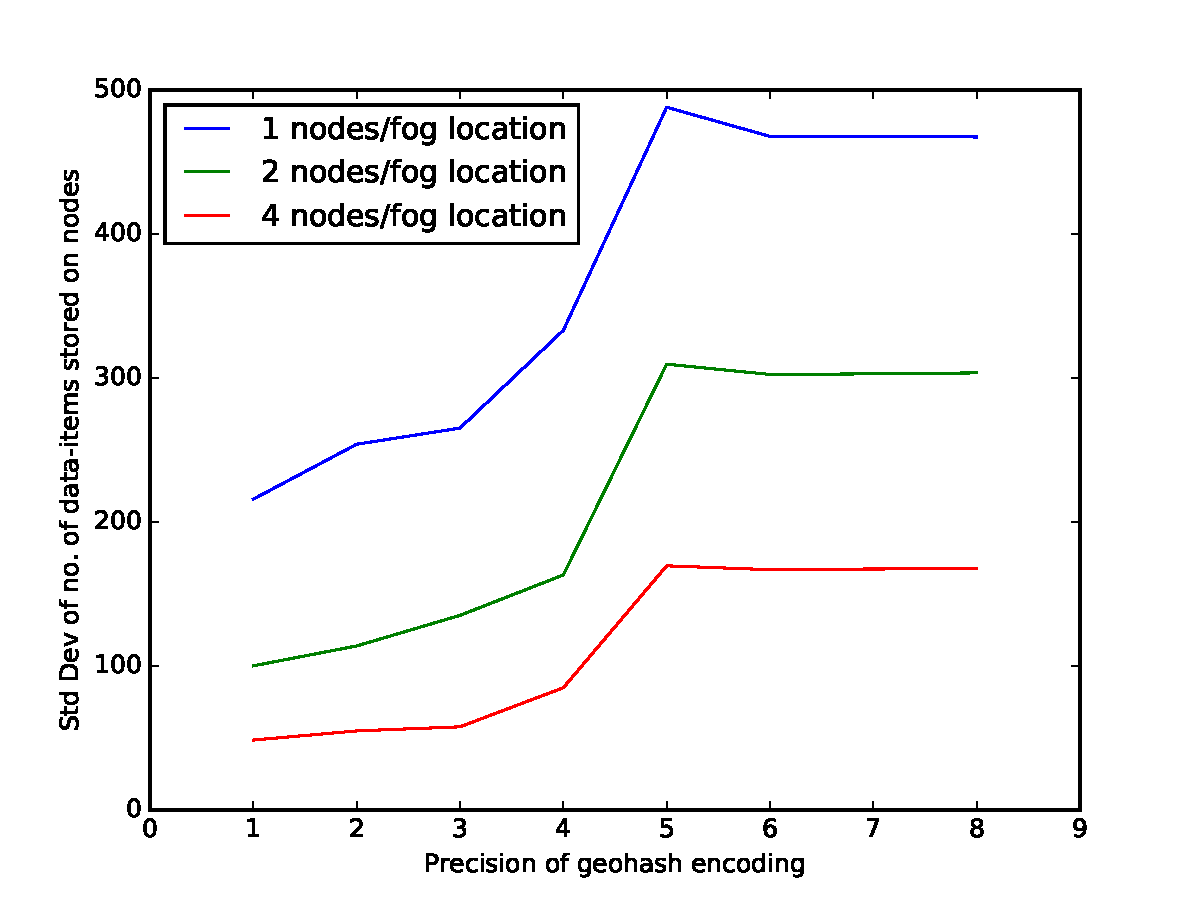
\includegraphics[width=0.75\columnwidth]{figures/fogstore/evals/hotspot/stdDevs.pdf}
\caption{Standard deviation of the number of data-items stored by each datastore node (lower number denotes better load balancing). We vary the precision used for Geohash encoding as well as the number of datastore nodes on each resource location. The numbers are averaged over 10 simulation runs.}
\label{fig:loadbalancing}
\end{figure}
\par As described in Section \ref{sec:implementation}, the precision of encoding a data-node's location for generating its token is crucial for determining the degree of spatial load balancing. A smaller value of precision leads to a large number of nodes having the same location-specific part of the token, leading to more widespread load balancing. A larger precision leads to higher spatial proximity and, hence, less widespread load balancing. We are able to see the above effect of Geohash encoding precision on the degree of load balancing (as show in Figure \ref{fig:loadbalancing}). Interestingly, a Geohash encoding precision of 5 and above encodes the location of all datastore nodes to be distinct, thus leading to no changes in load balancing metric for higher precision. 
\par Furthermore, an increase in the number of datastore nodes on each resource location also improves the load balancing metric, as the data-partitioning policy is able to seamlessly distribute data-items across them as well.  Hence with a proper precision of Geohash encoding for token formation and enough resources near regions with higher activity, we can obtain both spatial proximity of replicas and good load balancing.

\subsection{Evaluation of fault-tolerance}
One of the important properties of Fogstore's data distribution policy is that it takes tolerance to geographically correlated failures into account. Contemporary cloud-based databases provide such fault-tolerance by distributing replicas of a data-item across multiple datacenters, so that they are at a sufficiently high distance from each other to not be affected by correlated failures like earthquakes or massive power outages. Fogstore, however due to lack of physical constructs like datacenters and regions, performs wide-area geo-distribution using the location of data-items and data-store nodes, by guaranteeing a certain minimum distance in their spatial encodings. However, since spatial encodings tend to translate higher (two) dimensional attributes into one-dimension, high distance in terms of encoding of two locations does not consistently translate to high geographical (actual) distances between the two locations 
\par In the following set of experiments we examine the distribution that the geographical distance between Out-of-CoI replica nodes have from the data-item. Since the In-CoI replicas are kept close to the data-item's location, placing the Out-of-CoI replicas significantly far away from the data-item's location implies geographical separation between the In-CoI and Out-CoI replicas - thus achieving the aforementioned tolerance to correlated failures. We choose a few candidate large-scale resource topologies that are likely of being representative of how such geo-distributed infrastructures could be realized, which are described below :
\begin{enumerate}
\item Capitals : Each capital of mainland USA's states is considered a central location of resource capacity, with a fixed number of fog nodes scattered around a certain radius (50 km) from the capital city's centre.
\item AT\&T : Locations of core routers of AT\&T's backbone network inside the USA are considered central locations of resource capacity, with a fixed number of fog nodes scattered around a certain radius (50 km) from the peering points location.
\end{enumerate}
\par Accesses are generated from within a radius of 100 km from each central resource capacity location (an example of which is shown in Figure \ref{fig:faultToleranceTopo}).
\begin{figure}[h]
\centering
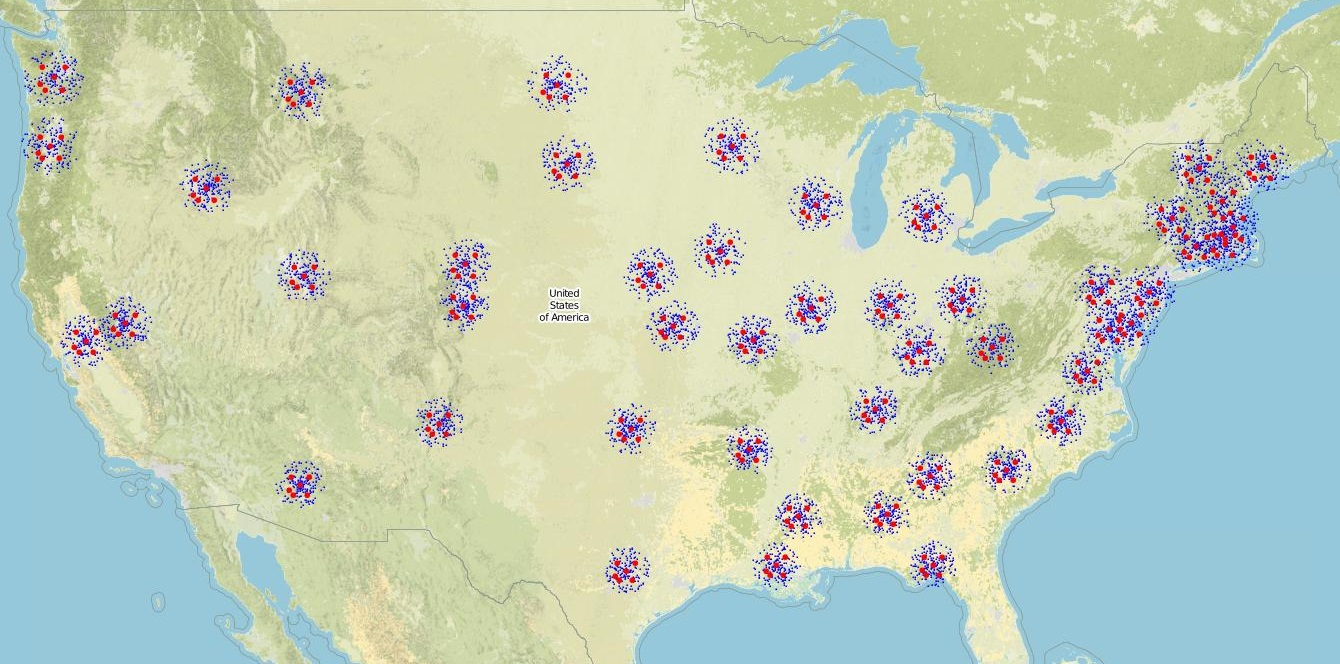
\includegraphics[width=0.75\columnwidth]{figures/fogstore/evals/fault-tolerance/map_accesses.jpg}
\caption{Geographical distribution of data-store resources (red dots) and accesses (blue dots) for a reference topology with mainland USA state capitals as resource capacity locations.}
\label{fig:faultToleranceTopo}
\end{figure}
We note the location where the Out-CoI replicas are placed and the distance of that node from the location of the data-item for the aforementioned reference topologies, as shown in Figure \ref{fig:outCoiDistance}. For both the candidate topologies, a maximum encoding distance threshold of 34 can allow a median separation of atleast 2500 KM, which is a significantly large distance for geographically-correlated failures, like natural disasters or massive power outages, to affect.
\begin{figure}[h]
\centering
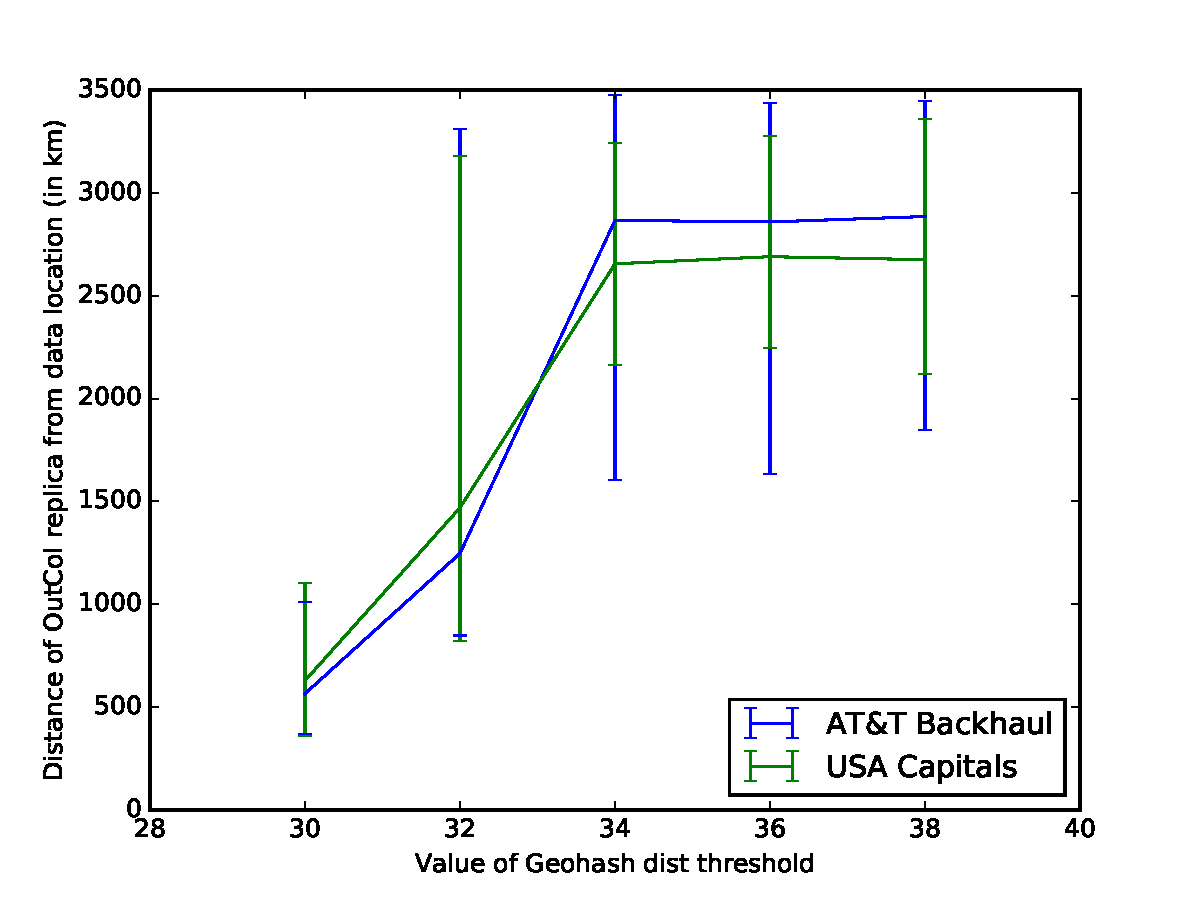
\includegraphics[width=0.75\columnwidth]{figures/fogstore/evals/fault-tolerance/outCoiDist.pdf}
\caption{Distribution of distance between OutCoI replicas and data-items' locations for various reference topologies. The precision of Geohash encoding for generating the token has been taken as 8.}
\label{fig:outCoiDistance}
\end{figure}

\section{Conclusion}
\label{sec:conclusion}
\begin{itemize}
\item 
\end{itemize}